\chapter{Results}\label{chap:results}

In this chapter, we will introduce the results of the experiments subjecting
protein representations to various relevant perturbation regimes highlighted in
chapter \ref{chap:methods}. We first discuss the results and implications of
frequently used \gls{mmd} configurations, namely by showing how it behaves
on protein graph descriptors. We then move on to show the results of the
sensitivity of the \gls{mmd} values depending on the underlying graph
representation used to extract the various graphs. Finally, we explore more
exotic configurations of \gls{mmd} that we hypothesize might be more
suitable for proteins. We conclude this chapter with a short section on the
runtimes of the various elements of the computational pipelines shown in this
chapter.

\section{Overall \gls{mmd} Behavior}\label{sec:overall_behaviour}

\subsection{General observations on the correlation
  coefficients}\label{sec:general_coefficients}
Surprisingly, we found that the behavior of \gls{mmd} was not as
inconsistent for the types of graphs extracted from proteins as was found on
synthetic graphs by \cite{obray2022evaluation}. Figure
\ref{fig:mmd_consistent_eps} show trajectories and correlations of
\gls{mmd} values with different perturbation types using
$\varepsilon$-graphs with $\varepsilon$ set to $8$ \si{\angstrom}. Both the
Spearman and Pearson correlation coefficients averaged across runs are high.
There is, however, an exception: the correlation between the \gls{mmd}
obtained from the degree histogram and the addition of edges is comparatively
low with $\rho_P=0.25$ and $\rho_S=-0.44$ versus that obtained from the
Laplacian spectrum histogram (with $\rho_P=0.95$, $\rho_S=0.98$), and the
clustering histogram (with $\rho_P=0.95$, $\rho_S=0.97$). Curiously, the next
lowest (Pearson) correlation coefficient from Figure
\ref{fig:mmd_consistent_eps} is also associated to the degree distribution
histogram under the rewiring perturbation regime ($\rho_p=0.82$ $\rho_S=0.98$).

\subsection{General observations on the standard deviations}\label{sec:general_std} In parallel, Table
\ref{tab:1_1_std} also supports the fact that the standard deviation of the
normalized \gls{mmd} of the degree distribution descriptor is the highest,
suggesting that this is not a very robust descriptor. Since modelling graph
connectivity is one of the primary challenges of generative graph models
\citep{li2018learning}, based on these results we do not recommend using a
degree histogram as a descriptor function for \gls{mmd}. The remaining
descriptors do show high correlations ($\rho_P\geq 0.89$, $\rho_S\geq 0.97$) and
reasonably low standard deviations ($>0.64$), which make them good candidates.

\begin{figure}[!htbp]
  \centering
  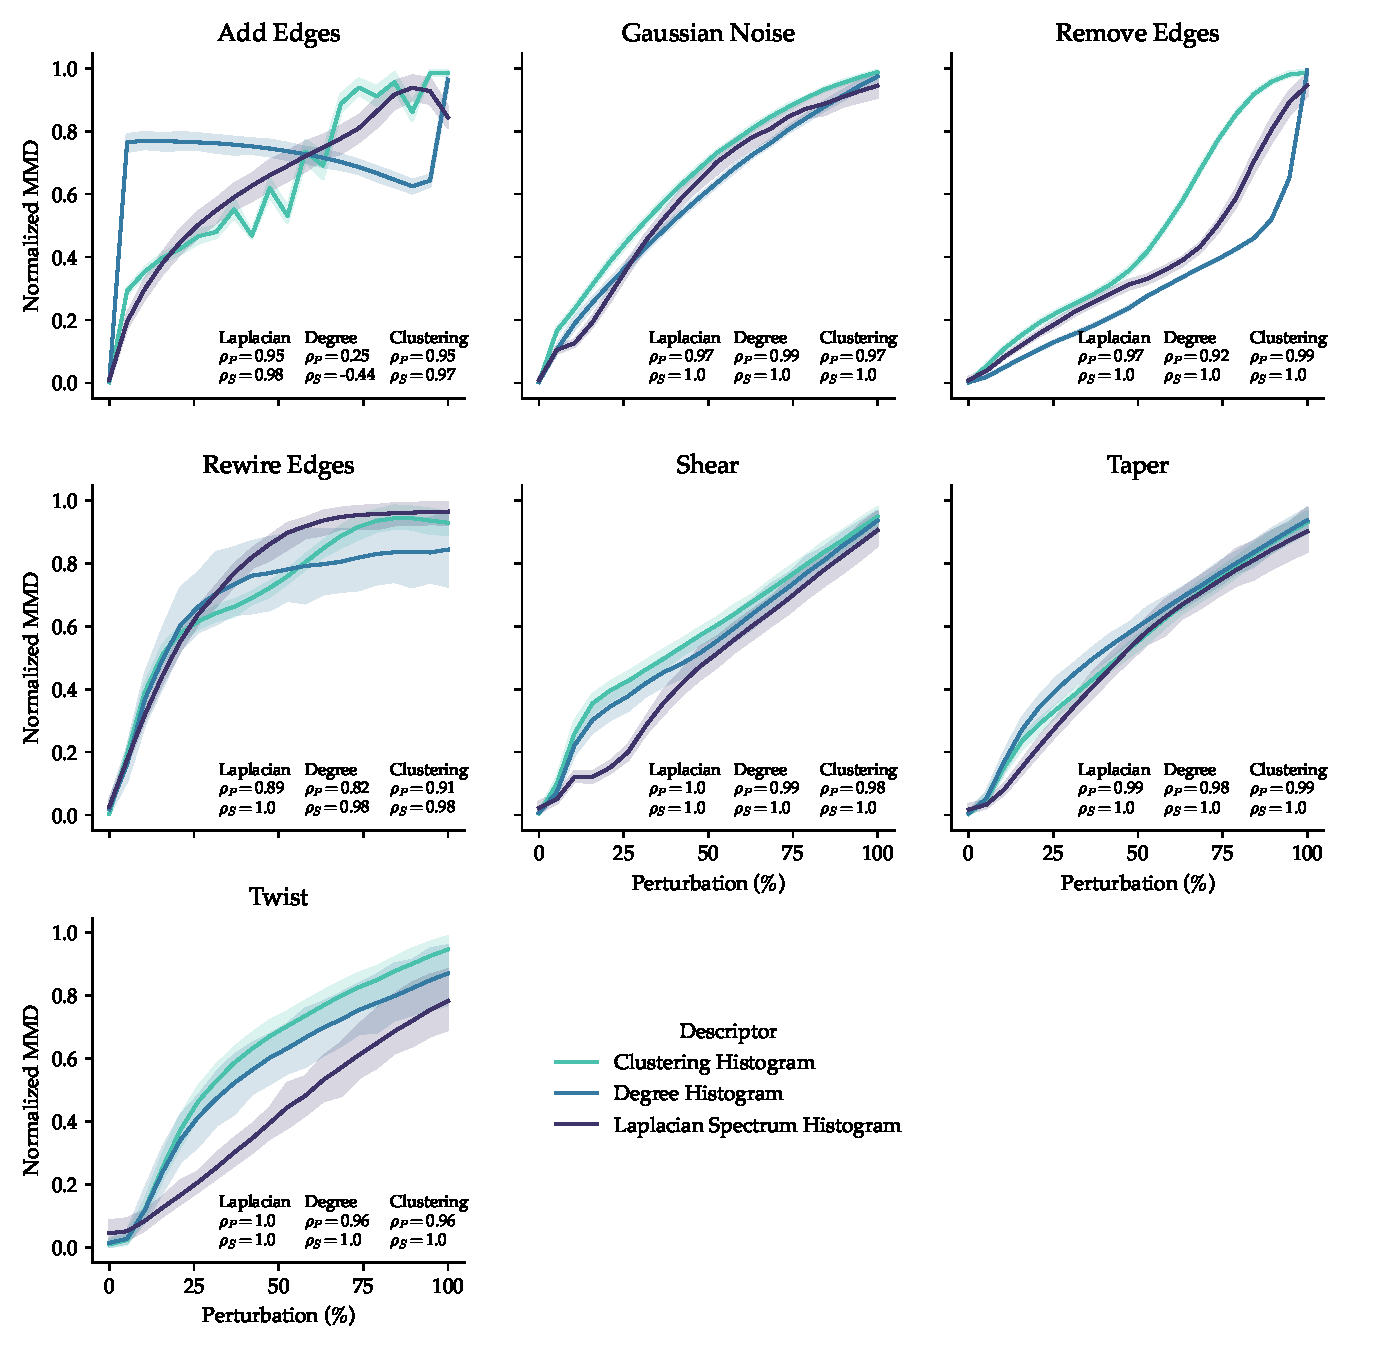
\includegraphics[width=\textwidth]{./figures/results/res_1_1.pdf}
  \caption[Overall behaviour of \gls{mmd} using graph-based
descriptors.]{\gls{mmd} vs. perturbation (in \% of the maximum values shown
  in Table \ref{tab:perturbation_ranges}) for various graph
descriptors of the 8\si{\angstrom}-graphs under different perturbations regimes.
The kernel used to obtain these graphs is the RBF kernel with bandwidth 0.01.
$\rho_{S}$: average Spearman correlation coefficient across runs. $\rho_{P}$:
average Pearson correlation coefficient across runs. Except for the degree
histogram behaviour when edges are added, we see that most \gls{mmd}
configurations behave well, i.e. there is a high correlation betweeen the
\gls{mmd} values and the perturbation.}
  \label{fig:mmd_consistent_eps}
\end{figure}

\begin{table}
  \centering
  \scalebox{0.75}{
  \begin{tabular}{llr}
    \toprule
    \textbf{Perturbation Type} & \textbf{Descriptor} & $\sigma_\MMD$ \\
    \midrule
Add Edges & Clustering Histogram &        0.023058 \\
      & Degree Histogram &        0.024943 \\
      & Laplacian Spectrum Histogram &        0.039320 \\
Gaussian Noise & Clustering Histogram &        0.010556 \\
      & Degree Histogram &        0.012793 \\
      & Laplacian Spectrum Histogram &        0.027411 \\
Remove Edges & Clustering Histogram &        0.009075 \\
      & Degree Histogram &        0.004400 \\
      & Laplacian Spectrum Histogram &        0.018033 \\
Rewire Edges & Clustering Histogram &        0.028672 \\
      & Degree Histogram &        \textbf{0.103612} \\
      & Laplacian Spectrum Histogram &        0.032276 \\
Shear & Clustering Histogram &        0.030793 \\
      & Degree Histogram &        0.041350 \\
      & Laplacian Spectrum Histogram &        0.040984 \\
Taper & Clustering Histogram &        0.025951 \\
      & Degree Histogram &        0.035282 \\
      & Laplacian Spectrum Histogram &        0.043468 \\
Twist & Clustering Histogram &        0.052784 \\
      & Degree Histogram &        0.081318 \\
    & Laplacian Spectrum Histogram &        0.063795 \\
    \bottomrule
  \end{tabular}
}
  \caption[Average standard deviation of the various \gls{mmd} configurations
  shown in Figure \ref{fig:mmd_consistent_eps} under the same perturbation
  types.]{Average standard deviation of the various \gls{mmd} configurations shown
    in Figure \ref{fig:mmd_consistent_eps} under the same perturbation
    types. The highest standard deviation is observed for the degree histogram
    descriptor under rewiring perturbations.}

  \label{tab:1_1_std}
\end{table}
% TODO: shave significant digits
\clearpage

\subsection{Influence of the choice of kernel}

We next investigate the overall influence of the kernel on the correlations
between perturbations and \gls{mmd} shown in Figure
\ref{fig:mmd_effect_kernel}. We can see that for $\sigma\lessapprox 0.1$
($\sigma$ being the hyperparameter of the Gaussian kernel, see Section
\ref{sec:kernels}) and for the linear kernel, \gls{mmd} values behave as
desired, i.e. $\rho_P, \rho_S\geq 0.8$ and, if one excludes the Laplacian
spectrum histogram at $\sigma=0.1$, we have $\rho_P,\rho_S>0.95$. However,
correlation coefficients drop sharply when increasing $\sigma>0.1$, most likely
due to oversmoothing, which is a phenomenon arising when the bandwidth of the
kernel is large enough to obscure any structure in the data
\citep{hwang1994nonparametric}. This can have unpredictable consequences on
resulting \gls{mmd} values: in the case of the degree histogram or the clustering
histogram, this results in an overly sensitive kernel sharply increasing in
value at the slightest perturbation, while the clustering histogram remains
oblivious to large amounts of perturbation. This can be explained by the
relative scale of each of the embeddings and their pairwise distances, which we
catalogue in Appendix \ref{sec:distance_dist}. % TODO: flesh this out a bit further maybe.

\begin{figure}[!htbp]
  \centering
  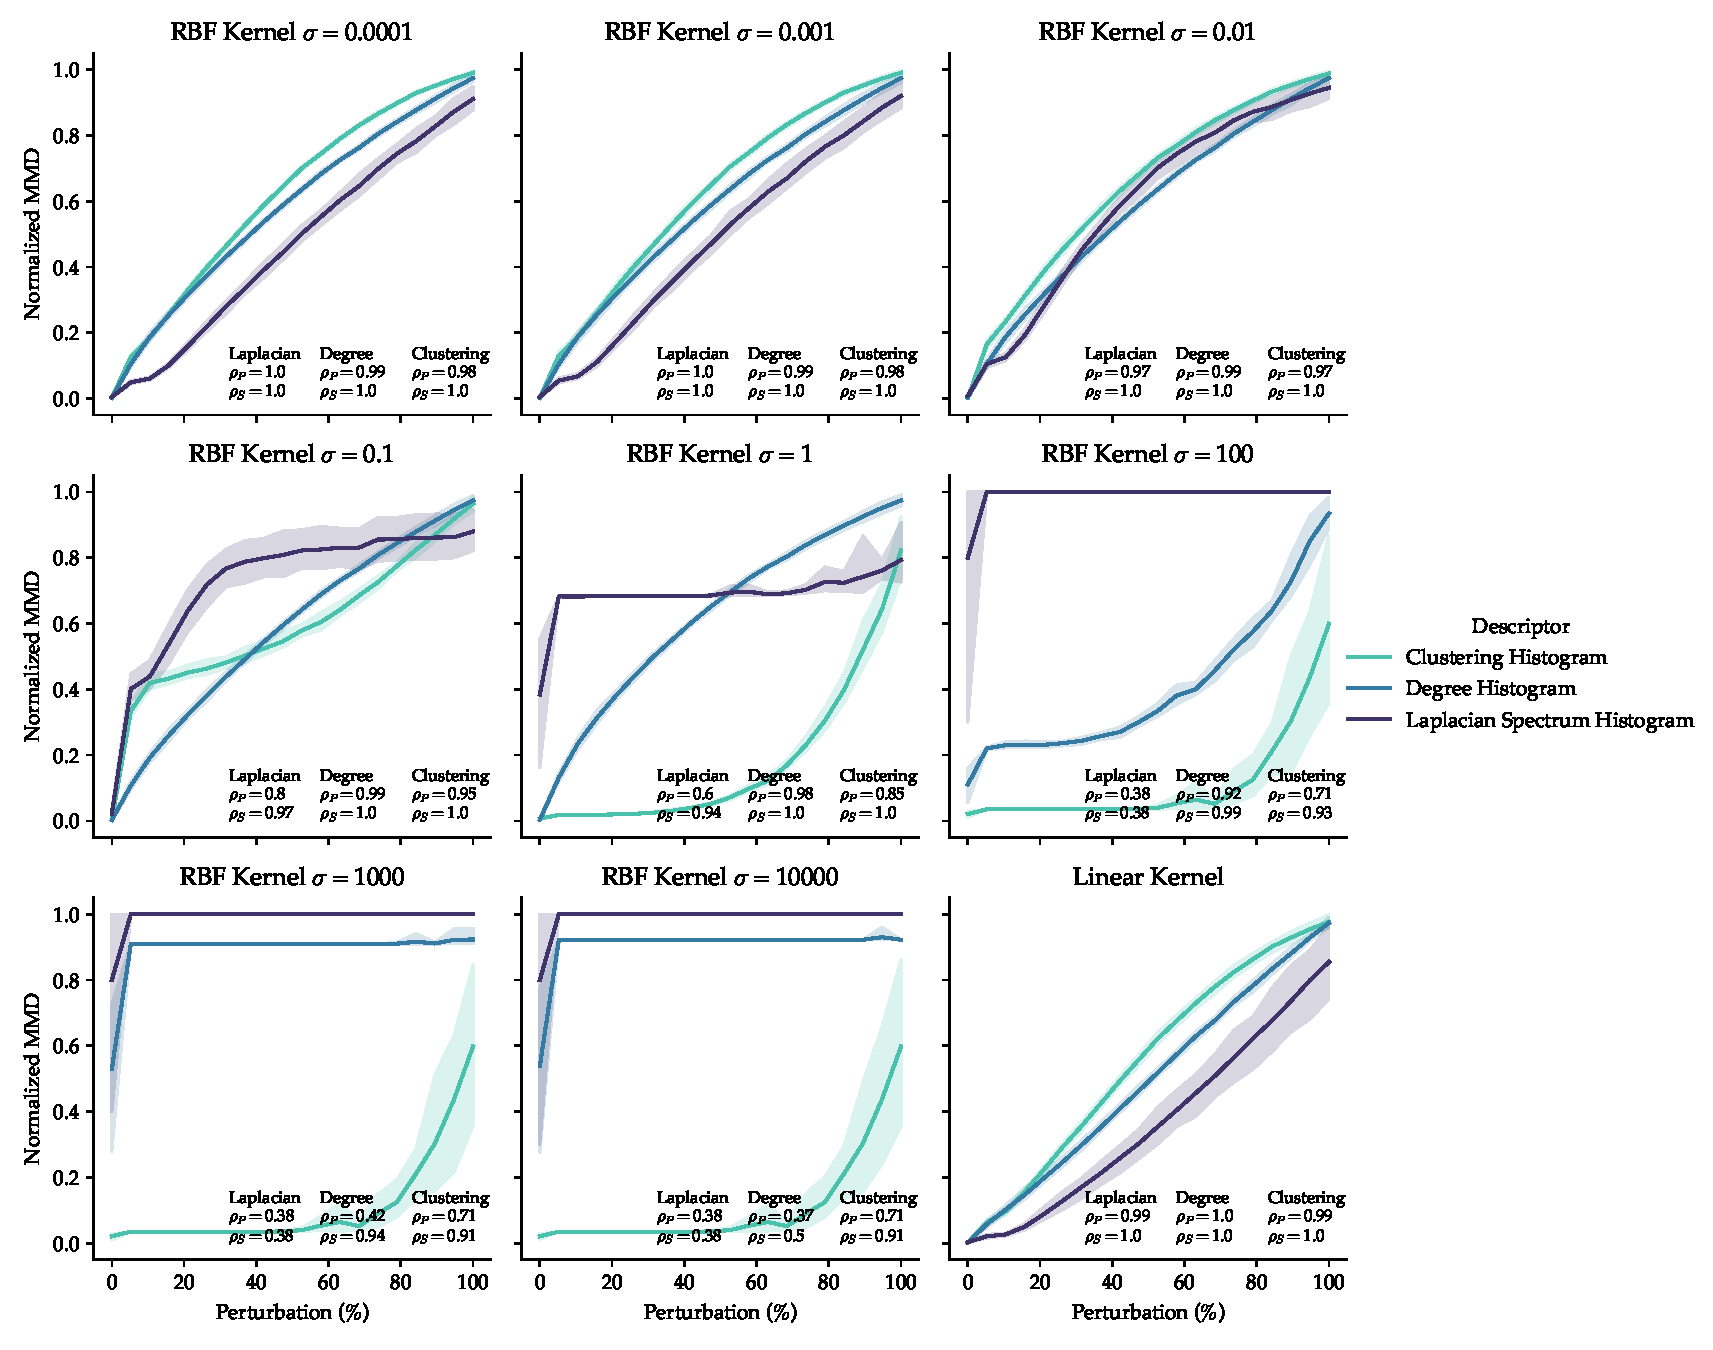
\includegraphics[width=\textwidth]{./figures/results/res_1_2.pdf}
  \caption[Influence of kernel parameters on \gls{mmd} behaviour.]{\gls{mmd} vs. Gaussian
    noise perturbation (in \% of the maximum values shown
    in Table \ref{tab:perturbation_ranges}) for various graph descriptors of the
    8\si{\angstrom}-graphs. $\rho_{S}$: average Spearman correlation coefficient
    across runs. $\rho_{P}$: average Pearson correlation coefficient across runs.
    The kernel here is shown on top of each subplots. We can see that reasonable
    behaviour of the RBF kernel can be seen when $\sigma<1$. The linear kernel also
    behaves well.}
  \label{fig:mmd_effect_kernel}
\end{figure}

\section{Influence of the Graph Representation on \gls{mmd}}\label{sec:results_sensitivity}

\subsection{Comparing Graph Construction Technique}\label{sec:techniques}
To compare which graph construction technique was overall most adviseable, we
computed the correlation coefficients of the various available combinations of
graph type, graph extraction parameter, and description function with an RBF
kernel with $\sigma=0.01$, which was shown to behave reasonably stably across
descriptors (Figure \ref{fig:mmd_effect_kernel}). We then compared the
distributions of the two correlation coefficients and computed a Mann-Whitney
$\mathcal{U}$ test \citep{fay2010wilcoxon}. Figure
\ref{fig:correlations_graph_construction} shows the distributions of both
$\rho_S$ and $\rho_P$ for the $k$-NN and $\varepsilon$-graphs. Both the test for
the Pearson correlation coefficient and the Spearman correlation coefficient
were significant ($p=8.35\cdot 10^{-4}$ and $p=1.765\cdot 10^{-2}$,
respectively) indicating that one distribution is stochastically greater than
the other. In both cases, the distribution of the correlation coefficients from
the $\varepsilon$-graphs is higher, as we can see in the legend of Figure
\ref{fig:correlations_graph_construction}. This result is intuitive, because
$\epsilon$-graphs are likely more sensitive to the underlying topology of the
protein. We therefore proceed with $\epsilon$-graphs in the subsequent results
discussed below.

\begin{figure}[!htbp]
  \centering
  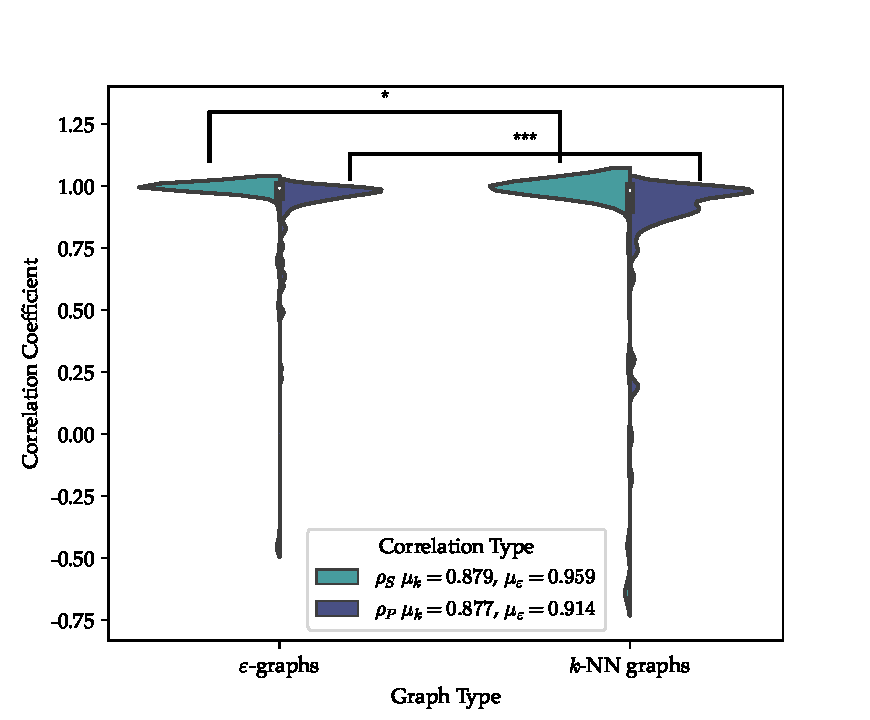
\includegraphics[width=0.8\textwidth]{./figures/results/compare_corrs_graph_construction.pdf}
  \caption[Violin plot of the distributions of the correlation coefficients of
various \gls{mmd} configurations derived from the two different graph
construction methods.]{Violin plot of the distributions of the correlation
coefficients of various \gls{mmd} configurations derived from the two
different graph construction methods. Each distribution contains various
combinations of descriptor functions, perturbation types, and various values of
the parameter used to extract the graphs (i.e. $k$ in the case of $k$-NN graphs
and $\varepsilon$ in the case of $\varepsilon$-graphs). The distributions are
then compared using a Mann-Whitney $U$ test, yielding significant $p$-values for
both $\rho_S$ and $\rho_P$ ($p=8.35\cdot 10^{-4}$ and $p=1.765\cdot 10^{-2}$,
respectively), indicating that the correlation coefficients obtained from $k$-NN
graphs are statisitcally significantly worse than those obtained from
$\varepsilon$-graphs. }
  \label{fig:correlations_graph_construction}
\end{figure}
% TODO: discuss the idea of the M-W U test with Tim

\subsection{Lower Values of $\varepsilon$ Are More Stable}
\label{sec:sparser_better}
In the previous paragraph, we established that $\varepsilon$-graphs were more
appropriate to compute the \gls{mmd}. Now, we investigate which specific
threshold(s) $\varepsilon$ are most appropriate using the same meta-metrics as
before. Figure \ref{fig:mmd_sensitivity_eps} shows the normalized \gls{mmd} values
with the varying degree of different types of perturbations with various graph
descriptors. While most configurations exhibit high correlations: excluding
seven outliers of the 72 coefficients calculated, we have $\rho_P>0.97$ and
$\rho_S>0.98$. In Figure \ref{fig:mmd_sensitivity_eps}, we can also see that
lower coefficients tend to be reached when using a high threshold $\varepsilon$.
For instance, in the case of the twisting perturbation and using the clustering
histogram as a graph descriptor, we see $\rho_P=0.73$ and $\rho_S=0.71$ for 32
\si{\angstrom}-graphs vs $\rho_P=0.96$ and $\rho_S=1.0$ for both 16 and 8
\si{\angstrom} graphs. While this is the most extreme example, we also see a
similar pattern when using a different descriptor, such as the Laplacian
spectrum histogram, where we have $\rho_P=\rho_S=0.93$ for 32\si{\angstrom}
graphs vs $\rho_P=0.99 \rho_S=1.0$ for 16\si{\angstrom} graphs and $\rho_P=1.0
\rho_S=1.0$ for 8-\si{\angstrom} graphs. While there are some exceptions to this
pattern, the differences are not nearly as substantial (the highest difference
where the correlation coefficient for the 32-\si{\angstrom} graph is higher than
the other two $\varepsilon$ thresholds is 0.03, see lower mid pane of Figure
\ref{fig:mmd_sensitivity_eps}).

The finding that increasing $\varepsilon$ decreases the overall quality of \gls{mmd}
is further supported by the changes in standard deviation of the different runs
averaged across the applied perturbation range, which is summarized in Table
\ref{tab:std_dev_epsilon_influence}. In this table, we can see that higher
values of $\varepsilon$ almost consistently incur a higher standard deviation,
i.e. we almost always have $\sigma_{\MMD, 32\si{\angstrom}}>\sigma_{\MMD,
  16\si{\angstrom}}>\sigma_{\MMD, 8\si{\angstrom}}$. The degree histogram descriptor under shearing
and tapering perturbations seems to be the two exceptions out of 12 cases.
Interestingly, the standard deviations were highest when subjecting proteins to
the twisting perturbation, most likely due to the fact that the spheres used to
construct the graphs most likely increasingly overlap when some degree of twist
is applied. In short, the conclusion of the last two paragraphs is that the
sparser the graph representation by lowering $\varepsilon$, the more stable the
resulting \gls{mmd}.
% TODO: change \gls{mmd} with acrshort.

\begin{figure}
  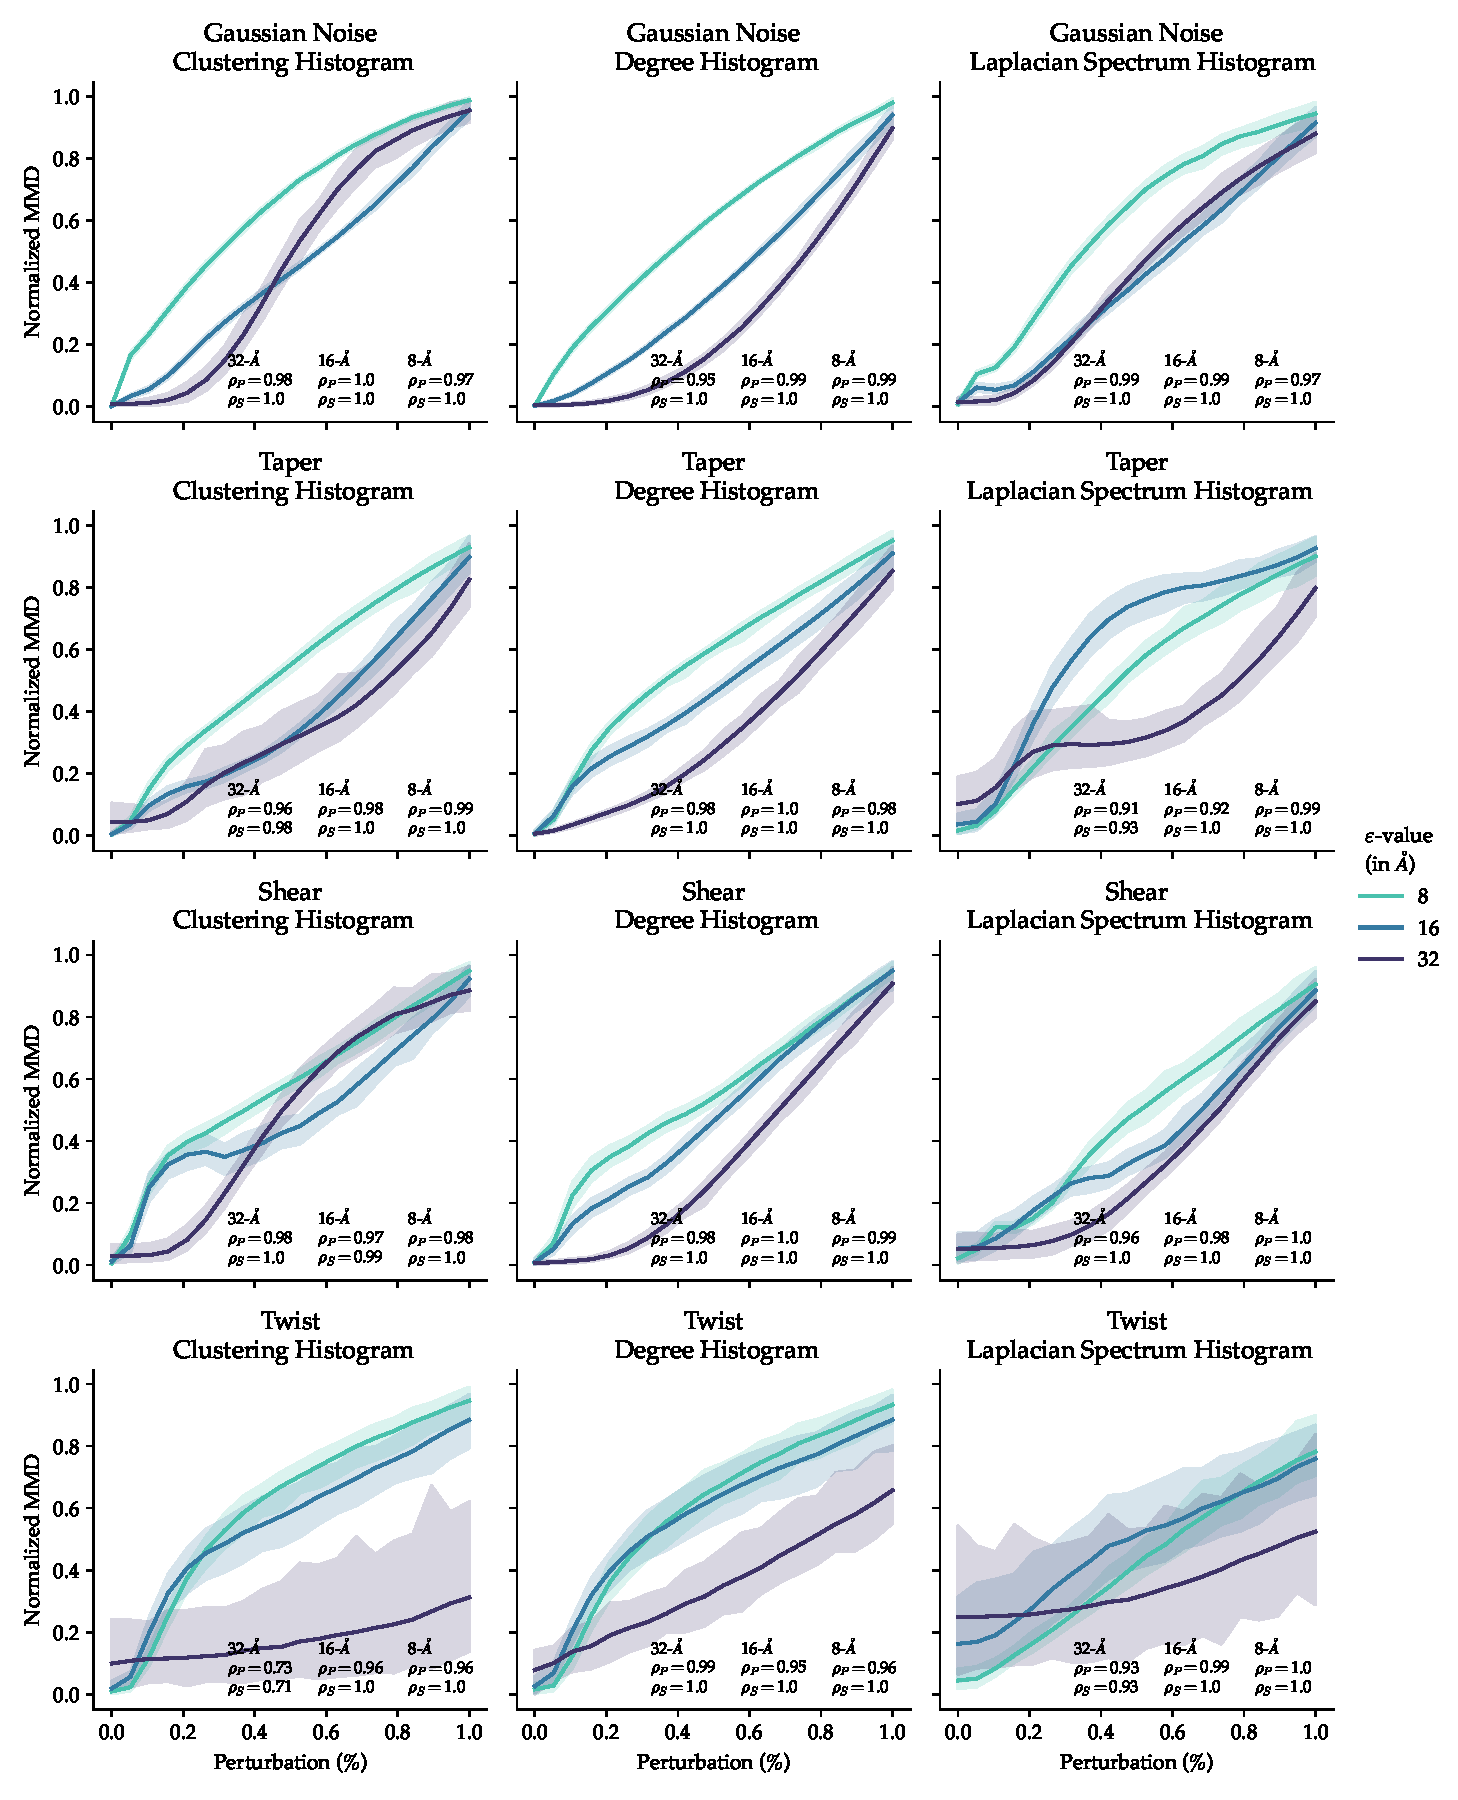
\includegraphics[width=\textwidth]{./figures/results/res_2_1.pdf}
  \caption[Influence of $\varepsilon$ on the sensitivity of \gls{mmd} to perturbations.]{\gls{mmd} vs. point cloud perturbation for various descriptors. In general,
when graphs are extracted with a lower $\varepsilon$ value, the \gls{mmd} curve
increases more rapidly. The only exception to this trend is the Laplacian
spectrum histogram descriptor under the tapering perturbation.}
  \label{fig:mmd_sensitivity_eps}
\end{figure}

\begin{table}
  \centering
  \scalebox{0.75}{
  \begin{tabular}{lllr}
    \toprule
    Perturbation Type & Descriptor Function & $\varepsilon$ & $\sigma_\MMD$ \\
    \midrule
    Gaussian Noise & Clustering Histogram & 8  &           0.011 \\
    &                              & 16 &           0.015 \\
    &                              & 32 &           0.043 \\
    & Degree Histogram & 8  &           0.013 \\
    &                              & 16 &           0.017 \\
    &                              & 32 &           0.024 \\
    & Laplacian Spectrum Histogram & 8  &           0.027 \\
    &                              & 16 &           0.030 \\
    &                              & 32 &           0.034 \\
    Shear & Clustering Histogram & 8  &           0.031 \\
    &                              & 16 &           0.049 \\
    &                              & 32 &           0.055 \\
    & Degree Histogram & 8  &           0.041 \\
    &                              & 16 &           0.038 \\
    &                              & 32 &           0.030 \\
    & Laplacian Spectrum Histogram & 8  &           0.041 \\
    &                              & 16 &           0.048 \\
    &                              & 32 &           0.050 \\
    Taper & Clustering Histogram & 8  &           0.026 \\
    &                              & 16 &           0.031 \\
    &                              & 32 &           0.088 \\
    & Degree Histogram & 8  &           0.035 \\
    &                              & 16 &           0.049 \\
    &                              & 32 &           0.044 \\
    & Laplacian Spectrum Histogram & 8  &           0.043 \\
    &                              & 16 &           0.053 \\
    &                              & 32 &           \textbf{0.089} \\
    Twist & Clustering Histogram & 8  &           0.053 \\
    &                              & 16 &           \textbf{0.082} \\
    &                              & 32 &           \textbf{0.179} \\
    & Degree Histogram & 8  &           \textbf{0.081} \\
    &                              & 16 &           \textbf{0.103} \\
    &                              & 32 &           \textbf{0.104} \\
    & Laplacian Spectrum Histogram & 8  &           0.064 \\
    &                              & 16 &           \textbf{0.145} \\
    &                              & 32 &           \textbf{0.229} \\
    \bottomrule
  \end{tabular}
}
\caption[Inter-run standard deviation values averaged across the whole
pertubation range for all combinations of perturbation type, descriptor
functions, and $\varepsilon$ values.]{Inter-run standard deviation values
averaged across the whole pertubation range for all combinations of perturbation
type, descriptor functions, and $\varepsilon$ values. Values higher than $0.08$
are in bold. Twisting perturbations show particularly high average standard
deviations $>0.05$, and higher $\varepsilon$ values also shows the highest
standard deviation values $>0.1$ for the twisting perturbations. In almost all
cases, we have $\sigma_{\MMD, 32-\AA}>\sigma_{\MMD, 16-\AA}>\sigma_{\MMD,
8-\AA}$. The degree histogram descriptor under shearing and tapering
perturbations seems to be the exceptions.}
  \label{tab:std_dev_epsilon_influence}
\end{table}


\subsection{Lower $\varepsilon$ Values for Graph Contruction Are More
Sensitive to Lower Perturbation Regimes}\label{sec:sensitivity}
While we noted that choosing a lower $\varepsilon$ value
to extract the graph would likely improve the stability of resulting \gls{mmd}s, there
is also another consideration when choosing a graph representation. As shown in
Figure \ref{fig:mmd_sensitivity_eps}, when 20\% of the maximum amount of
perturbation applied\footnote{See Table \ref{tab:perturbation_ranges} for the
respective maxima.}, in seven out of 12 cases, the normalized \gls{mmd} of
8\si{\angstrom} graphs is higher than that of the 16- or 32 \si{\angstrom} graphs. In
addition, we find that, generally, in lower perturbation regimes, higher
percentages of the normalized \gls{mmd} are reached with graphs constructed with a
lower $\varepsilon$. Figure \ref{fig:difference_sensitivity_20_percent}
illustrates this phenomenon. By grouping each configuration of \gls{mmd} under
different perturbation types at the 20\% mark of the maximum perturbation
applied, we see that the 8\si{\angstrom}- and 16\si{\angstrom} graphs are
significantly higher than that of the 32\si{\angstrom} graphs (Mann-Whitney
$\mathcal{U}$ test: $p=1.08\cdot 10^{-4}$ and $p=5.56\cdot 10^{-3}$,
respectively). In short, in addition to being overall more stable, lower
$\varepsilon$ values and sparser subsequent graphs also tend to be better at
detecting smaller changes in protein topologies than larger $\varepsilon$ values
and denser graphs. This is useful for a practitioner in advanced stages of
modeling, where small changes in the generated graph population need to be
detected.


\begin{figure}
  \centering
  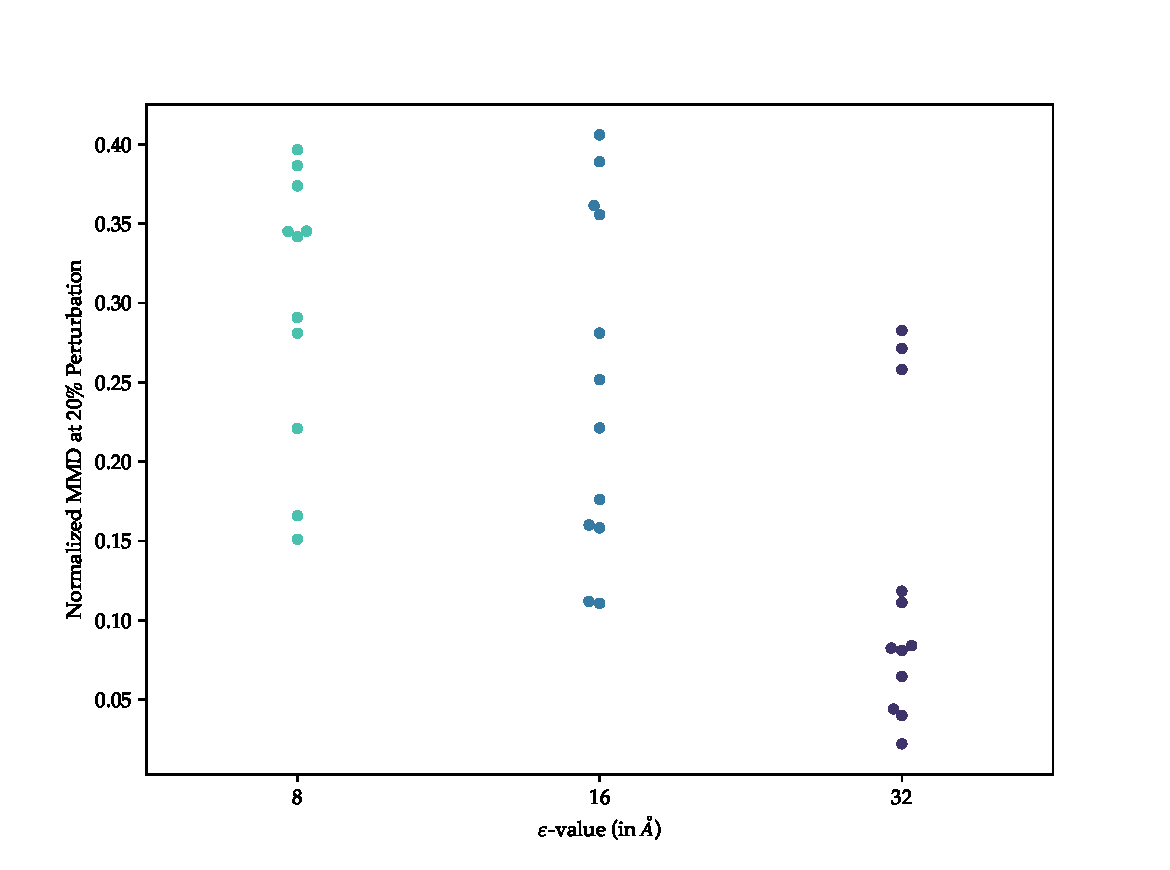
\includegraphics[width=\textwidth]{./figures/results/swarmplot_2_1.pdf}
  \caption[Normalized \gls{mmd} value at 20\% of the maximum perturbation amount for
various \gls{mmd} configurations at different $\varepsilon$ values.]{Normalized \gls{mmd}
value at 20\% of the maximum perturbation amount (as shown in Table
\ref{tab:perturbation_ranges}) for various \gls{mmd} configurations at different
$\varepsilon$ values. The difference between the 8\si{\angstrom}- and
32\si{\angstrom} graphs is significant (Mann-Whitney $\mathcal{U}$-test
$p=1.08\cdot 10^{-4}$). The difference between the 16\si{\angstrom}- and
32\si{\angstrom} graphs is also significant ($p=5.56\cdot 10^{-3}$). However,
the difference between the 8\si{\angstrom}- and 16\si{\angstrom} graphs was not
signicant ($p=3.47\cdot 10^{-1}, 5\cdot 10^{-2}$ is our highest significance
threshold.)}
  \label{fig:difference_sensitivity_20_percent}
\end{figure}

\clearpage



% TODO: the sparser, the better?

% Among these outliers, we also see that the correlations are
% substantially lower when perturbing proteins with the twisting perturbation for
% the 32-\si{\angstrom}-graphs (the lowest are $\rho_P=0.73$ and $\rho_S=0.71$
% when using the clustering histogram as a graph descriptor).
% The overall quality
% of the \gls{mmd} configurations with various $\varepsilon$ thresholds can be further
% assessed using the standard deviation of the \gls{mmd} values across runs over the
% range of perturbations applied, which we summarize in Table
% \ref{tab:std_dev_epsilon_influence}. From

% we see that twisting
% perturbations show particularly high average standard deviations $>0.05$, and
% higher $\varepsilon$ values also show higher standard deviation values
% (culminating above $0.1$ for the twisting perturbation) for the twisting perturbations. In almost all cases, we have
% $\sigma_{\MMD, 32-\AA}>\sigma_{\MMD, 16-\AA}>\sigma_{\MMD, 8-\AA}$. The degree
% histogram descriptor under shearing and tapering perturbations seems to be the
% exceptions.


% TODO: erase/rewrite

% In the last section, we discussed the notion of sensitivity of a particular
% \gls{mmd} configuration to perturbations. We explore this idea further
% here. Specifically, we investigate the impact of the $\varepsilon$ threshold on
% the resulting sensitivity of the \gls{mmd} configuration to various
% perturbations affecting the underlying point cloud. Figure
% \ref{fig:mmd_sensitivity_eps} shows that, in general, the lower the
% $\varepsilon$, the more sensitive the \gls{mmd} to perturbations. Low
% sensitivity to perturbation might be useful in the early stages of modeling when
% generated samples only need to \emph{coarsely} match the reference samples.
% Conversely, a higher sensitivity to perturbations might be useful when trying to
% \emph{finely} distinguish a set of anomalous samples from the reference samples.
% Additionally, we can see that under the Gaussian noise, twisting and tapering
% perturbation, larger values of $\varepsilon$ introduce larger variations in
% \gls{mmd} values.



\section{Graph Kernels}\label{sec:results_graph_kernels}
% TODO compare WL with ESM (no modelling bias for WL on paper, might be a
% weakness since some mutations might not have a functional effect.)

The results of the perturbation experiments using the Weisfeiler-Lehman kernel
(see Sections \ref{sec:kernels} and \ref{sec:methods_kernels}) in \gls{mmd} can be
seen in Figure \ref{fig:wlk}. Two important takeaways can be be derived from
this figure.

% TODO: WL glossary entry
\subsection{Quality of \gls{mmd} Using Weisfeiler-Lehman}\label{sec:quality_wl}
The first conclusion is
derived from the observation of the meta metrics. We can see that, correlations
are relatively low for graph perturbations (Figure \ref{fig:wlk}, top row). If
we take the kernel using 5 iterations for instance, we get $\rho_P=0.4$ and
$\rho_S=0.44$ when adding edges. Additionally, from the shape of the curve, we
can also derive that the Weisfeiler-Lehman kernel is not sensitive to changes in
the number of edges unless an extreme amount is added. Removing edges also
results in a similar curve, but correlation coefficients are higher, with
$\rho_P=0.68$ and $\rho_S=1.0$ ( $\rho_P$ is still considerably lower than other
configurations of \gls{mmd} examined thus far, see earlier Sections
\ref{sec:overall_behaviour} and \ref{sec:results_sensitivity} for details). The
next perturbation (rewiring edges), highlights the need for the standard
deviation estimation of different samples (see Table
\ref{tab:std_graph_kernel}), because although the correlation coefficients are
reasonable ($\rho_P=0.71$, $\rho_S=0.99$), one could realistically not
distinguish highly rewired protein graphs from another, because $\sigma_\MMD$ is
extremely high compared to other configurations or other types of perturbations
(for the rewiring, all $\sigma_\MMD>0.28$ while the other $\sigma_\MMD<0.15$).
This reflects the high confidence internal we see in the upper right pane of
Figure \ref{fig:wlk}. For point cloud perturbations, correlation coefficients
are in line with the coefficients we have seen before ($\rho_P>0.94$ and we
consistently have $\rho_S=1$), there seems to be a crucial caveat in the curves
that we see in Figure \ref{fig:wlk} which we discuss next.

\subsection{Insensitivty in Low Perturbation Regimes} \label{sec:insensitivity_wl_kernel}
Figure \ref{fig:wlk} indeed reveals a systematic pathology when using the
Weisfeiler-Lehman kernel in \gls{mmd}. When applying a low amount of perturbation,
there does not seem to be a proportional rise in the (normalized) \gls{mmd} value. As
an example, the normalized \gls{mmd} only rises substantially from the observed value
on the unperturbed set after adding 10\% of Gaussian noise to the data (which
corresponds to 3.16\si{\angstrom}, see Figure
\ref{fig:perturbation_illustration} for an illustration of what 10\% of Gaussian
noise looks like for a given protein). This `inverted elbow' shape of the curve
seen in almost all perturbation types except for the rewiring regime, where the
very high $\sigma_\MMD$ seems to obscure any meaningful pattern as discussed in
the previous paragraph. This phenomenon is particularly pronounced in the other
two graph perturbation scenarios, where 80\%-95\% of the perturbation needs to
be added to observe any meaningful change in \gls{mmd}. This has dramatic implications
for practitioners, as this means that one cannot distinguish between a generated
sample of graphs and a real one unless the generated sample exhibits highly
pathological features, which is undesirable for evaluation purposes. While the
reason for these findings are not entirely clear, it is possible that the
diversity of the hashes obtained during the Weisfeiler-Lehman algorithm is so
high that substantial changes need to occur prior to observing any shifts in the
dot product of the resulting hash histograms. Further analyses on the diversity
of hashes and their relative population needs to be done to validate this
hypothesis. Another way to remedy this pathology would be to not use the amino
acid as node labels. While this would entail loosing sensitivity to mutations,
the diversity of hashes might be substantially reduced so as to ensure that the
resulting dot products will be more sensitive to changes in hash populations.


% Contrary to the tendencies observed in Section
% \ref{sec:results_sensitivity}, \gls{mmd}s obtained using the
% Weisfeiler-Lehman kernels on 8\si{\angstrom} graphs are very \emph{insensitive} to
% medium levels of perturbations (the resulting curves only start to increase
% anywhere starting from 5\% to 85\% of the perturbation range), and seems to even completely oblivious to rewiring of
% graphs and generally insensitive to graph perturbations unless highly perturbed
% (see upper row of Figure \ref{fig:wlk}).


% The most likely explanation is that the
% diversity of Weisfeiler-Lehman hashes (i.e. neighborhoods) observed within
% perturbed or unperturbed samples is relatively high, which makes distinguishing
% between the two a high threshold to overcome. This drawback could disappear if
% one is working on a more targeted set of morphologically similar proteins with a
% lower diversity of Weisfeiler-Lehman hashes, but this is beyond the scope of the
% thesis.

\begin{figure}
  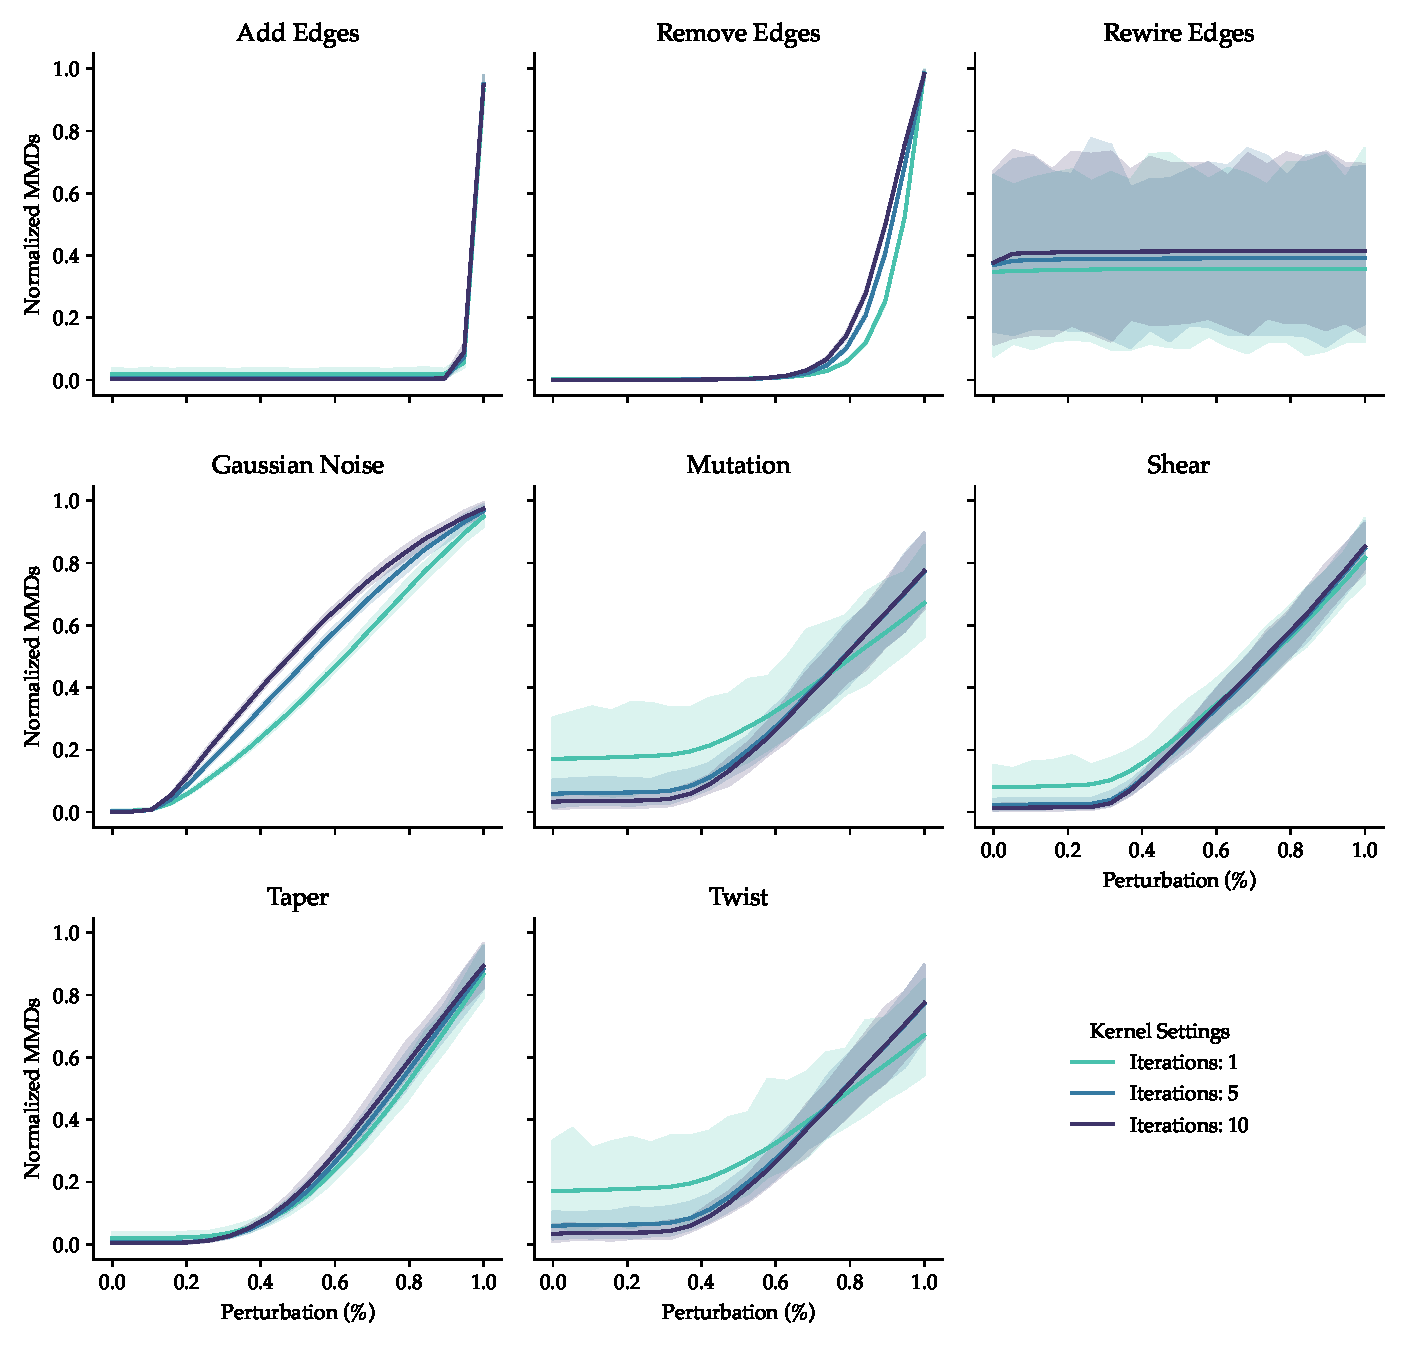
\includegraphics[width=\textwidth]{./figures/results/res_3.pdf}
  \caption[Normalized \gls{mmd} values using the Weisfeiler-Lehman kernel subject to
  various perturbations.]{\gls{mmd} vs.
perturbations using the Weisfeiler-Lehman kernel using the
8\si{\angstrom}-graphs as inputs. We see that high levels of perturbations are
required to raise the normalized \gls{mmd} values. We also see that \gls{mmd}s computed with
the Weisfeiler-Lehman kernel are insensitive to the rewiring of edges, and
results in \gls{mmd}s with a high inter-run variance.}
  \label{fig:wlk}
\end{figure}


\begin{table}
  \centering
  \scalebox{0.75}{
  \begin{tabular}{llr}
    \toprule
    \textbf{Perturbation Type} & \textbf{Iterations} & $\sigma_\MMD$ \\
    \midrule
    Add Edges & Iterations: 1 &           0.018 \\
    & Iterations: 5 &           0.007 \\
    & Iterations: 10 &           0.006 \\
    Gaussian Noise & Iterations: 1 &           0.016 \\
    & Iterations: 5 &           0.014 \\
    & Iterations: 10 &           0.013 \\
    Mutation & Iterations: 1 &           \textbf{0.147} \\
    & Iterations: 5 &           0.072 \\
    & Iterations: 10 &           0.061 \\
    Remove Edges & Iterations: 1 &           0.004 \\
    & Iterations: 5 &           0.003 \\
    & Iterations: 10 &           0.004 \\
    Rewire Edges & Iterations: 1 &           \textbf{0.296} \\
    & Iterations: 5 &           \textbf{0.290} \\
    & Iterations: 10 &           \textbf{0.287} \\
    Shear & Iterations: 1 &           0.079 \\
    & Iterations: 5 &           0.046 \\
    & Iterations: 10 &           0.043 \\
    Taper & Iterations: 1 &           0.037 \\
    & Iterations: 5 &           0.030 \\
    & Iterations: 10 &           0.029 \\
    Twist & Iterations: 1 &           \textbf{0.147} \\
    & Iterations: 5 &           0.072 \\
    & Iterations: 10 &           0.061 \\
    \bottomrule
  \end{tabular}
  }
  \caption{Standard deviations of the various Weisfeiler-Lehman configurations
under different perturbation regimes. Values higher than 0.1 are in bold.
Rewiring edges results in the highest standard deviations by far with
$\sigma_\MMD>0.28$. Lower iterations of the algorithm also results in higher
standard deviations.}
  \label{tab:std_graph_kernel}
\end{table}


\section{Protein-Specific Descriptors Are Inexpensive, High-Quality Descriptor
Functions}\label{sec:results_protein_descriptors}

Figure \ref{fig:protein_specific_descriptors} shows the normalized \gls{mmd} as
various types of perturbations are added to one set of proteins, where each row
has a corresponding perturbation type. Each column also corresponds to a
different kernel and kernel parameter configuration.

\subsection{Dihedral Angles Histograms}\label{sec:res_dihedral_angles}
We start our examination of the novel, protein-specific descriptors outlined in
Section \ref{sec:descriptors} by discussing the dihedral angles histograms of
the \textphi{} and \textpsi{} bond angles. We see that for this descriptor, the
kernel choice heavily influences the correlation coefficients; indeed, if one
chooses the linear kernel or the RBF kernel with a low bandwidth ($10^{-5}$) or
the parameter-free linear kernel, we obtain high correlation coefficients
($\rho_P>0.95$ and $\rho_S=1$) if we exclude the Gaussian noise perturbation,
which we discuss below. Indeed, correlation coefficients are low for this
descriptor when subject to Gaussian noise ($0.41>\rho_P>0.39$ and
$0.59>\rho_S>0.5$). While their associated standard deviation is not
particularly high (see Table \ref{tab:protein_descriptors_std}), this would
indicate that they would not be useful for use in \gls{mmd}.

However, when examining the profile of the perturbation curve (Figure
\ref{fig:protein_specific_descriptors}, top row), we can see that with very low
Gaussian noise levels (as low as 5\%, which in this thesis corresponds to
1.5\si{\angstrom}, see Table \ref{tab:perturbation_ranges}), the \gls{mmd} already
reaches its highest point. This phenomenon entails that the dihedral angles
histogram is not necessarily an inappropriate descriptor, but a very sensitive
one. This can be useful to practitioners; indeed, when predicting the 3D
structure of proteins from the amino acid sequence for instance,
\cite{jumper2021highly} had to apply an additional refinement algorithm
leveraging Amber force fields \citep{hornak2006comparison} to ensure that the
bond geometries were not violated (see \citep{jumper2021highly} p. 586 for a
detailed discussion). Such a descriptor used in \gls{mmd} can therefore provide
statistical evidence to support the statement that (generated) bond geometries
follow a natural distribution.

One conclusion additional conclusion from the analysis of this particular
protein descriptor is that although both Pearson and Spearman correlation
coefficients as well as $\sigma_\MMD$ provide powerful quantitative tools to
gauge the quality of a metric, i.e. meta-metrics, one should still carefully
consider the profile of individual perturbation experiments as well as reason
through the expressive power of a particular descriptor or kernel to accurately
assess the practicality of a particular \gls{mmd} configurations.

% TODO:

\subsection{\textalpha{}-Carbon Distance Histogram}\label{sec:results_dist_hist}

The distance histogram also serves as a good protein descriptor, and does not
exhibit some of the sensitivity-related pathologies that we discussed in Section.
\ref{sec:res_dihedral_angles}. If we set aside the twisting perturbation, which
we discuss below, we get high correlation coefficients ($\rho_P>0.97$ and
$\rho_S>0.99$ irrespective of the kernel or perturbation type chosen). Standard
deviations are also reasonably low, since we consistently have $\sigma_\MMD<0.1$
not considering twisting.

The \textalpha{}-carbon distance histogram descriptor as used in \gls{mmd} does not
seem to behave well under twisting perturbations, with both low correlations and
high standard deviations. While the RBF kernel configurations seem to have a
high correlation ($\rho_P,\rho_S\geq 0.95$), using the linear kernel yields
correlation coefficients as low as $\rho_P=0.35$ and $\rho_P=0.37$.
Additionally, the standard deviation for the \gls{mmd} curves obtained using the
\textalpha{}-carbon distance histogram descriptor are high across kernel choices
($\sigma_\MMD>0.22$), which does not make it a very robust descriptor.

While less sensitive than the dihedral angles descriptor, the
\textalpha{}-carbon distance histogram descriptor still provides several
advantages over the dihedral angles histogram. Although we have not tested
this here, this descriptor can certainly be used to accurately gauge the size in
3D space of the proteins generated. This can be useful when crafting generative
models that generate proteins conditioned on overall size in 3D space.
Additionally, as reflected through the different perturbations shown in Figure
\ref{fig:protein_specific_descriptors}, this descriptor is mostly able to detect
changes in the interatomic space. This can also allow a practitioner to detect
atom clashes and overall unrealistic distances in a protein model, much like the
atom clash detection steps in the PDB validation pipeline \citep{read2011new,
gore2012implementing, gore2017validation}. This could be further validated by
progressively increasing the distance of each atom from the center of mass of
the proteins.

\begin{figure}[htpb!]
  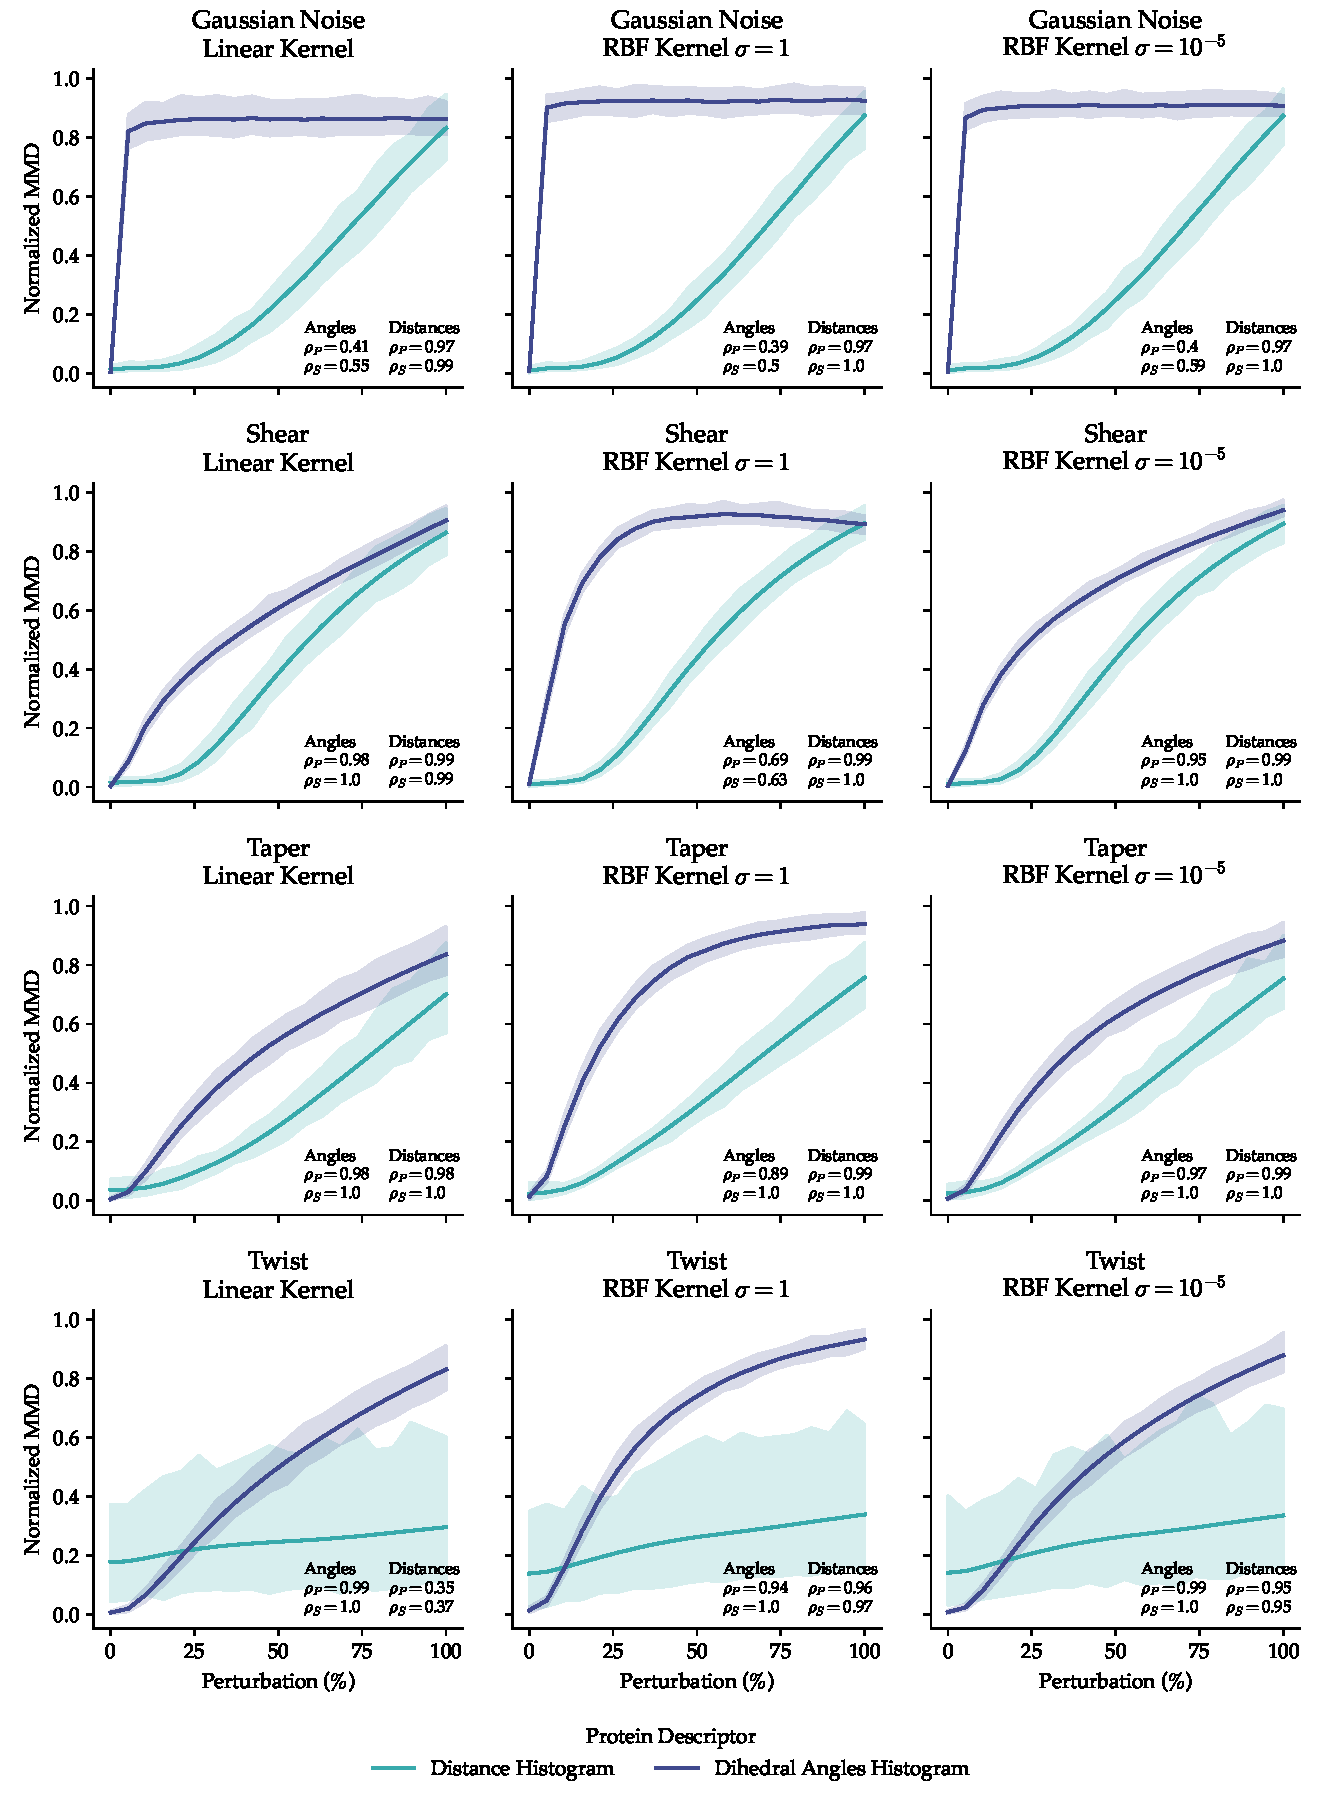
\includegraphics[width=\textwidth]{./figures/results/res_4.pdf}
  \caption[\gls{mmd} vs. perturbations using the two novel protein
descriptors.]{\gls{mmd} vs. perturbations (in \% of the maximum values
shown in Table \ref{tab:perturbation_ranges}) using the two novel protein
descriptors shown in Section \ref{sec:descriptors}. Each row has a corresponding
perturbation type. Each column also corresponds to a different kernel and kernel
parameter configuration. Those descriptors behave very well overall, with the
dihedral angles descriptors being particularly sensitive to Gaussian noise. The
distance histogram exhibits higher inter-run variance when subject to twisting
pertubations.}
  \label{fig:protein_specific_descriptors}
\end{figure}


\begin{table}
  \centering
  \scalebox{0.75}{
    \begin{tabular}{lllr}
      \toprule
      \textbf{Perturbation Type} & \textbf{Kernel} & \textbf{Descriptor} &  $\sigma_\MMD$ \\
      \midrule
      Gaussian noise & Linear Kernel & Dihedral Angles Histogram &           0.062 \\
                    &             & Distance Histogram &           0.071 \\
                    & RBF Kernel ($\sigma=1$) & Dihedral Angles Histogram &           0.048 \\
                    &             & Distance Histogram &           0.059 \\
                    & RBF Kernel ($\sigma=1\cdot 10^{-5}$) & Dihedral Angles Histogram &           0.042 \\
                    &             & Distance Histogram &           0.060 \\
      Shear & Linear Kernel & Dihedral Angles Histogram &           0.037 \\
                    &             & Distance Histogram &           0.066 \\
                    & RBF Kernel ($\sigma=1$) & Dihedral Angles Histogram &           0.035 \\
                    &             & Distance Histogram &           0.050 \\
                    & RBF Kernel ($\sigma=1\cdot 10^{-5}$) & Dihedral Angles Histogram &           0.028 \\
                    &             & Distance Histogram &           0.051 \\
      Taper & Linear Kernel & Dihedral Angles Histogram &           0.059 \\
                    &             & Distance Histogram &           0.079 \\
                    & RBF Kernel ($\sigma=1$) & Dihedral Angles Histogram &           0.040 \\
                    &             & Distance Histogram &           0.062 \\
                    & RBF Kernel ($\sigma=1\cdot 10^{-5}$) & Dihedral Angles Histogram &           0.049 \\
                    &             & Distance Histogram &           0.063 \\
      Twist & Linear Kernel & Dihedral Angles Histogram &           0.060 \\
                    &             & Distance Histogram &           \textbf{0.250} \\
                    & RBF Kernel ($\sigma=1$) & Dihedral Angles Histogram &           0.039 \\
                    &             & Distance Histogram &           \textbf{0.228} \\
                    & RBF Kernel ($\sigma=1\cdot 10^{-5}$) & Dihedral Angles Histogram &           0.050 \\
                    &             & Distance Histogram &           \textbf{0.230} \\
      \bottomrule
    \end{tabular}
  }
  \caption[Standard deviation of the various protein-specific descriptors
devised in this thesis.]{Standard deviation of the various protein-specific
descriptors devised in this thesis. $\sigma_\MMD>0.2$ are in bold. This table
reflects two observations made from Figure
\ref{fig:protein_specific_descriptors}: first, that overall standard deviation
of the \gls{mmd} values across the perturbation range is quite low. Second, the
distance histogram seem to result in particularly high standard deviations when
subject to twisting perturbations.
}
  \label{tab:protein_descriptors_std}
\end{table}

\section{\gls{mmd} from Learned Embeddings}\label{sec:results_esm}

As we noted in Section \ref{sec:kernels}, the only constraint on some of the
input vectors is that they need to be in $\R^d$. Additionally, as noted at the
end of Section \ref{sec:insensitivity_wl_kernel}, there has been much progress
in the development of learned embeddings. Finally, due to some of the
shortcomings of the Weisfeiler-Lehman kernel highlighted in Section
\ref{sec:insensitivity_wl_kernel}, we wanted to investigate the representative
power of learned embeddings in \gls{mmd}, the result of which are shown in Figure
\ref{fig:esm_descriptor}. In this figure, we see that choosing an RBF kernel
with $\sigma\leq 0.01$ or a linear kernel results in excellent correlation
coefficients with $\rho_P=0.94$ and $\rho_S\geq 0.96$ across kernels with
$\sigma\leq 0.01$. The standard deviation of the \gls{mmd} across this range of
kernels is also reasonable, with $\sigma_\MMD<0.1$ across the linear kernel and
RBF kernel with $\sigma<0.1$ (see Table \ref{tab:std_esm} for details). Further
work should focus on different kinds of perturbations applied to sequences and
see if correlation coefficients stay consistent across kernel configurations.
Results conducted by \cite{kucera2022conditional} suggest that this is not the
case, highlighting the need for further work.

% TODO: discuss kucera and more in-depth work on evaluating generative sequence models.

\begin{figure}
  \centering
  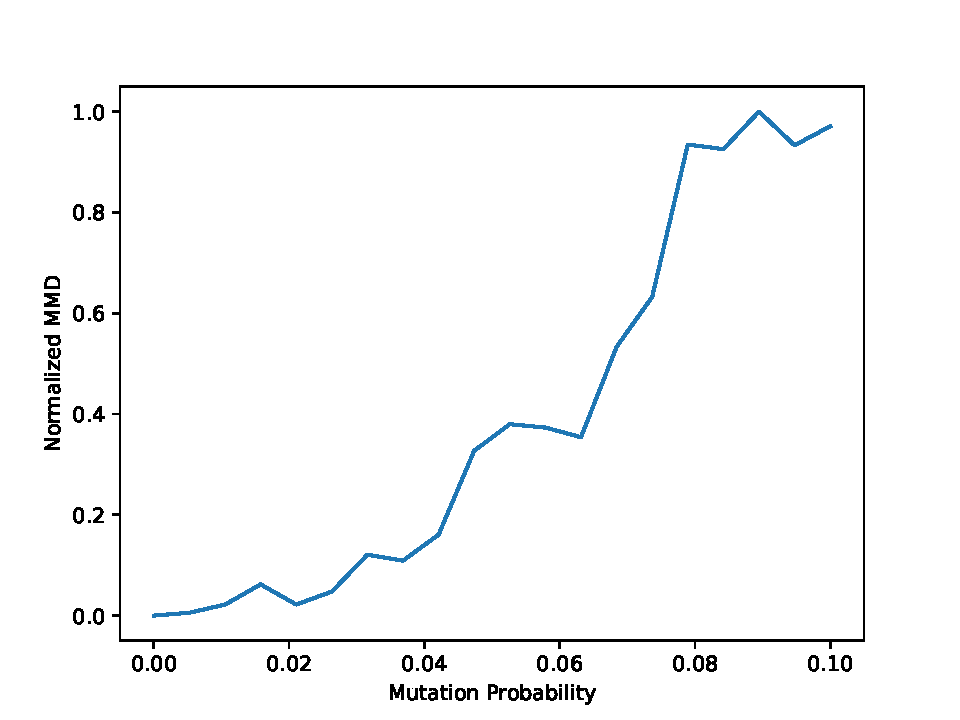
\includegraphics[width=\textwidth]{./figures/results/res_5.pdf}
  \caption[\gls{mmd} using \acrshort{esm} embeddings.]{\gls{mmd} vs. mutation probability using the \acrshort{esm}
learned embeddings with various kernels. The correlation coefficients of the
resulting \gls{mmd}s with RBF kernels with $\sigma<1$ and the linear kernel are high,
therefore making them good configurations for sequences. This analysis should be
complemented by complementary sequence-specific perturbations -- see Section
\ref{sec:discussion_realistic_proteins} for details.}
  \label{fig:esm_descriptor}
\end{figure}

\begin{table}
  \centering
  \scalebox{0.75}{
  \begin{tabular}{lr}
    \toprule
    \textbf{Kernel} & $\sigma_\MMD$  \\
    \midrule
    Linear Kernel &           0.091 \\
    RBF ($\sigma=1e-05$)   &           0.089 \\
    RBF ($\sigma=0.0001$)  &           0.092 \\
    RBF ($\sigma=0.001$)   &           0.093 \\
    RBF ($\sigma=0.01$)    &           0.093 \\
    RBF ($\sigma=0.1$)     &           0.095 \\
    RBF ($\sigma=1$)       &           \textbf{0.235} \\
    RBF ($\sigma=10.0$)    &           \textbf{0.447} \\
    \bottomrule
  \end{tabular}
  }
  \caption[$\sigma_\MMD$ values for the \gls{mmd} using the ESM learned
embedding.]{$\sigma_\MMD$ values for the \gls{mmd} using the ESM learned embedding.
$\sigma_\MMD>0.1$ are in bold. These findings corroborate the correlation
coefficients shown in Figure \ref{fig:esm_descriptor}: using a linear kernel or
an RBF kernel with$\sigma<0.1$, we get $\sigma_\MMD<0.1$, we obtain higher
quality (here, more robust) metrics, since $\sigma_\MMD$ is relatively low.}
  \label{tab:std_esm}
\end{table}

\clearpage

\section{Topological Descriptors and Kernels}\label{sec:results_topo_kernels}

% TODO kernel acronyms, \gls{tda} acronyms
Figure \ref{fig:tda_kernels} shows the behavior of both the \gls{msk}
and \gls{pfk}. Overall, we can see that they are among the best
performing metrics in this thesis, with high correlations and low inter-run
variation. The \gls{pfk} seems to perform the best based on the
correlation coefficients, with $\rho_P>0.95$ and $\rho_S=1$ across perturbation
types -- while the the \gls{msk} shows $\rho_P>0.93$ and $\rho_S>0.99$.
The \gls{pfk} also has slightly lower $\sigma_\MMD$ values than
the \gls{msk} with $\sigma_\MMD$, with a maximum of 0.024 vs 0.044 for
the \gls{msk} -- see Table \ref{tab:std_tda}. Additionally, when
looking at each perturbation type, we seem to have $\sigma_{\MMD
  ,\,\text{PSK}}<\sigma_{\MMD,\,\text{MSK}}$ except for the tapering
perturbation type, where there is a 0.02 difference $\sigma_{\MMD
,\,\text{PSK}}<\sigma_{\MMD,\,\text{MSK}}$. These differences in kernel
performance are minor, however, and both kernels perform consistently really
well compared to the alternative configurations explored in this thesis. Another
last finding related to the difference between the two kernels is that with
identical bandwidths and perturbation level, the MSK seems to be consistently
higher than the PFK. Therefore, if a more sensitive \gls{mmd} configuration is
required, the MSK might be preferred.

While the current \gls{tda} workflow cannot detect changes in node labels in the current setting, hence
not being able to detect mutations, we will show in Section
\ref{sec:tda_limitations} how this could be alleviated. For computational
reasons, we did not compute variations of different kernel parameters, although
one could speed up the operation by precomputing the kernel matrices, and only
subsequently multiplying the matrix by different constants (i.e. implement a
modified version of the speed up trick explored in Appendix A.5 of
\cite{obray2022evaluation}).

\begin{figure}
  \centering
  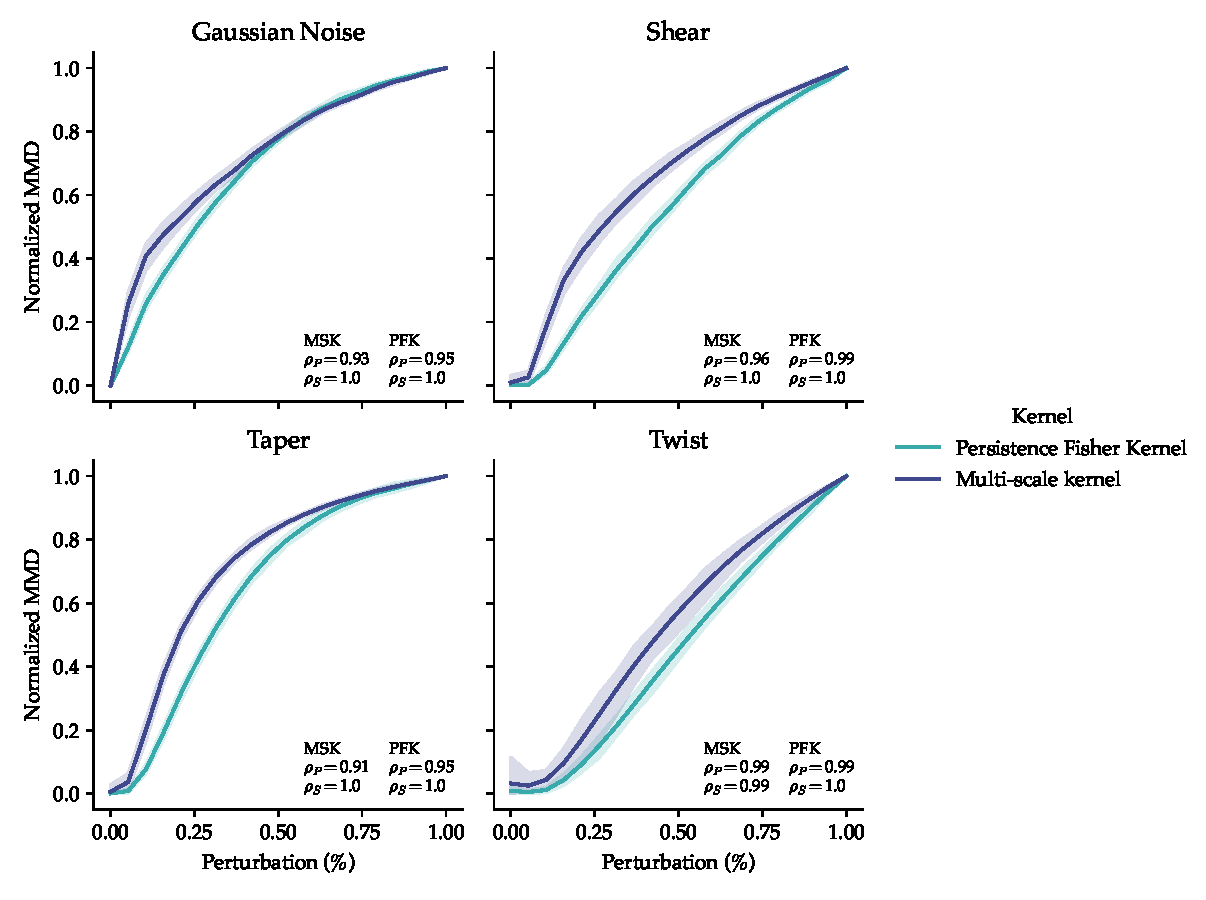
\includegraphics[width=\textwidth]{./figures/results/res_6.pdf}
  \caption[\gls{mmd} using topological kernels.]{\gls{mmd} vs. Perturbation (in
\% of the maximum values shown in Table \ref{tab:perturbation_ranges}) using the
\gls{msk} and persistence Fisher kernel. For the \gls{pfk}, both the
kernel bandwidth parameter and the Fisher bandwidth parameter are set to 1. For
the \gls{msk} (MSK), the bandwidth parameter is also set to 1. Overall,
the correlation coefficients for those kernels are very high and show little
inter-run variance, which is also supported by the $\sigma_\MMD$ values in Table
\ref{tab:std_tda}.}
  \label{fig:tda_kernels}
\end{figure}

\begin{table}
  \centering
  \scalebox{0.75}{
    \begin{tabular}{llr}
      \toprule
      \textbf{Perturbation Type} & \textbf{Kernel} & $\sigma_\MMD$ \\
      \midrule
      gaussian\_noise & Multi scale kernel &           0.017 \\
      & Persistence Fisher Kernel &           0.013 \\
      shear & Multi scale kernel &           0.025 \\
      & Persistence Fisher Kernel &           0.016 \\
      taper & Multi scale kernel &           0.014 \\
      & Persistence Fisher Kernel &           0.016 \\
      twist & Multi scale kernel &           0.044 \\
      & Persistence Fisher Kernel &           0.024 \\
      \bottomrule
    \end{tabular}
  }
  \caption[$\sigma_\MMD$ values for the \gls{mmd} using the persitence Fisher kernel
  and the multi scale kernel]{$\sigma_\MMD$ values for the \gls{mmd} using the persitence Fisher kernel (PSK)
    and the multi scale kernel (MSK).}
  \label{tab:std_tda}
\end{table}

% \section{Inter-Run Variance}

% In Figures \ref{fig:mmd_consistent_eps} through \ref{fig:tda_kernels}, we mostly
% commented on the correlation coefficients between the (normalized) \gls{mmd} values
% and the amount perturbation applied. While a high correlation is certainly a
% good indicator of a particular \gls{mmd} configuration, one should also carefully
% consider the (normalized) inter-run variance observed between independent
% samples of proteins. We can see that in Figures \ref{fig:mmd_consistent_eps}
% through \ref{fig:tda_kernels}, this variance changes quite a lot depending on
% the \gls{mmd} configuration. It can be high for certain representations.
% For instance in Figure \ref{fig:mmd_sensitivity_eps}, one can see that a higher
% $\varepsilon$ value (e.g. 32\si{\angstrom}) show a higher inter-run variance
% compared to a lower $\varepsilon$ value (e.g. 8\si{\angstrom}), when
% it comes to the twisting perturbation (lowest row). Furthermore, one of the
% descriptors devised for this thesis also exhibits high variance under twisting
% perturbations: the pairwise distance histogram, Figure
% \ref{fig:protein_specific_descriptors}. The consequence of a high normalized
% inter-run variance can be just as nefarious as \gls{mmd} configurations with low
% correlation coefficients because the range of absolute \gls{mmd} values can be too wide
% to make an accurate assessment of the quality of generated samples.

\clearpage
\section{Runtime}\label{sec:results_runtime}

% TODO add numbers. Maybe big-O.
One of the desiderata of \gls{mmd} is efficiency, i.e. a low computational
complexity (see Section \ref{sec:evalproblem}). As such, we report the various
computation times for each of the important elements of the pipelines outlined
in this thesis. The summary of all execution times can be found in Table
\ref{tab:runtimes}.

First, we see that one computation stands out: computing the Vietoris-Rips
filtration of a point cloud. Together with a large memory footprint, the
Vietoris-Rips filtration is expensive to compute (3332s in our benchmarks), due
to a runtime of $\mathcal{O}(n^{3(k+2)})$, where $k$ is the number of dimensions
(here, $k=3$) and $n$ the number of points \citep{adams2018persistent}. Although
some optimizations have been carried out by \texttt{Ripser}
\cite{Bauer2021Ripser}, the software used to compute the Vietoris-Rips
filtration, it remains very expensive to compute and does not enjoy the benefits
of hardware acceleration through e.g. a GPU due to the difficulty of
parallelizing such a filtration.

Second, computing the distance histogram and dihedral angles histogram are the
fastest descriptors to compute (28s for the former and 4s for the latter),
making them suitable to evaluate large collections of generated proteins. Other
graph descriptors are also reasonably fast to compute (35-175s in our
benchmarks, see Table \ref{tab:runtimes}), but they depend on the settings used
to extract the graphs, and, generally, the runtime increases in the number of
edges of the graph.

Third, the kernels used in this study all have reasonable runtimes, but we note
the particular efficiency of the RBF and linear kernel ($<7.7$ms in our
benchmarks) compared to the persistence Fisher, multi-scale and
Weisfeiler-Lehman kernel. In addition, the \gls{pfk} ran thee
times slower (35s) than the \gls{msk} (11s). The implications of these
runtimes will be further explored when making recommendations to the practioner
in Section \ref{sec:discussion_recommendations}.


\begin{table}
  \centering
  \begin{tabular}{lll}
    \toprule
    \textbf{Operation} &  \textbf{Execution Time} \\
    \midrule
    \textbf{Descriptor Functions} & \\
    \midrule
    Vietoris-Rips Filtration & 3332 s \\
    \acrshort{esm} Embedding & 163 s\\
    Degree Distribution Histogram (32\si{\angstrom}-graph) & 35 s\\
    Clustering Coefficient Histogram (32\si{\angstrom}-graph) & 175 s\\
    Laplacian Spectrum Histogram (32\si{\angstrom}-graph) & 35 s\\
    Distance Histogram & 28 s\\
    Dihedral Angles Histogram & 4 s\\
    \midrule
    \textbf{Kernels} & \\
    \midrule
    Weisfeiler-Lehman Kernel (4 iterations) & 32 s \\
    Persistence Fisher Kernel & 35 s \\
    Multi-Scale Kernel & 11 s \\
    RBF Kernel  & 1.7 ms \\
    Linear Kernel  & 7.7 ms \\
    \bottomrule
  \end{tabular}
  \caption[Runtime and computational complexity of the various elements of the
  pipeline.]{Runtime and computational complexity of the various elements of the
pipeline. These timings are obtained by executing the operation on 100 samples
spread across 10 CPU cores from an Intel Xeon Gold 6254 CPU clocked at 3.10GHz.}
  \label{tab:runtimes}
\end{table}


\clearpage

\section{Summary}

In this chapter, we present the results of the behavior of \gls{mmd} under
various configurations and subject to different types of perturbations. We start
by examining the graph descriptors used in the literature to evaluate generative
graph models (\ref{sec:overall_behaviour}). For those descriptors, we notice
that the correlation coefficients generally behave well, with the exception of
the degree histogram, which shows lower correlations and in some cases higher
standard deviations, making it the least expressive and robust of all
descriptors for graph representations of proteins (Section
\ref{sec:general_coefficients} and \ref{sec:general_std}). We also examined the
influence of the choice of kernel, and observed that the RBF kernel with
$\sigma<0.1$ and the linear kernel showed high correlation coefficients, but
that those coefficients drop sharply when increasing $\sigma>0.1$, which likely
due to the scale of the various descriptors, and for which increasing $\sigma$
results in oversmoothing (Section \ref{sec:general_coefficients}). We then
investigated the quality of the extracted graphs following different graph
extraction techniques and parameters (Section \ref{sec:results_sensitivity}). In
Section \ref{sec:techniques}, we established that $\varepsilon$-graphs were
often better to use based on the correlation coefficient distribution. Next, in
Section \ref{sec:sparser_better}, we established that lower $\varepsilon$ values
yielded more stable \gls{mmd} configurations. To wrap up our
discussion of the combinations of descriptor and kernel traditionally used in
the literature, we concluded in Section \ref{sec:sensitivity} that at lower
perturbation regimes, higher values of the normalized \gls{mmd} were reached by graphs
constructed with a lower $\varepsilon$ threshold.

We then moved on to our discussion of the Weisfeiler-Lehman kernel, which is a
kernel operating directly on graphs, and noted it's low relative quality
compared to \gls{mmd} configured with graph descriptors, both in terms of correlation
and standard deviation (Section \ref{sec:quality_wl}). Further, we noted no
increase in normalized \gls{mmd} in low regimes of perturbation for \gls{mmd}s configured
with the Weisfeiler-Lehman kernel \ref{sec:insensitivity_wl_kernel}.

Next, we examined the protein-specific descriptor functions that we devised for
use in \gls{mmd} (Section \ref{sec:results_protein_descriptors}). We found that both
the dihedral angles (Section \ref{sec:res_dihedral_angles}) and the distance
histograms (\ref{sec:results_dist_hist}) were appropriate protein descriptors,
although they investigate different aspects of the protein topology (bond angles
and interatomic distances, respectively).

We briefly examined sequence embeddings in Section \ref{sec:results_esm} and
although the early mutation results seem promising, more work needs to be done
to properly assess \gls{mmd} configurations applied to sequences.

We discuss the last set of \gls{mmd} configurations in Section
\ref{sec:results_topo_kernels}, where we find that kernels operating on
persistence diagrams tend to work exceptionally well to capture point cloud
perturbations. We noted that the MSK was slight more sensitive (i.e. the
resulting \gls{mmd}s were consistently higher for this kernel at any given
perturbation level) and but slightly less well performing than the PFK in terms
of correlation and standard deviation, although those differences were minor.

Finally, we conclude this chapter with a summary of the runtime of the various
elements of the computational pipleine to obtain \gls{mmd} values (Section
\ref{sec:results_runtime}), and note that (i) the Vietoris-Rips filtration is
excessively slow to compute, (ii) that the protein descriptors are particularly
fast to compute, and (iii) comment on the various kernel runtimes.

% TODO: introduce next chapter?
